\documentclass[tikz,border=7pt]{standalone}
\usepackage{libertinus}
\usepackage{amsmath}
\usetikzlibrary{
  arrows.meta,
  backgrounds,
  calc,
  decorations.markings,
  fit,
  positioning
}

\definecolor{accent}{RGB}{38,103,115}
\definecolor{softgray}{RGB}{244,245,246}
\definecolor{midgray}{RGB}{123,128,132}

\tikzset{
  >={Latex[length=2.2mm,width=1.5mm]},
  flow/.style={-Latex,semithick,draw=black!72},
  accent flow/.style={-Latex,semithick,draw=accent},
  box/.style={
    draw=black!68,
    fill=softgray,
    rounded corners=1.2pt,
    align=center,
    inner xsep=5pt,
    inner ysep=4pt
  },
  accent box/.style={
    draw=accent,
    fill=accent!8,
    rounded corners=1.2pt,
    align=center,
    inner xsep=5pt,
    inner ysep=4pt
  },
  point/.style={circle,draw=black!75,fill=white,inner sep=1.7pt},
  accent point/.style={circle,draw=accent,fill=accent!10,inner sep=1.7pt},
  tinylabel/.style={font=\scriptsize,align=center},
  smalllabel/.style={font=\small,align=center},
  panel/.style={draw=black!28,rounded corners=2pt,inner sep=6pt}
}


\begin{document}
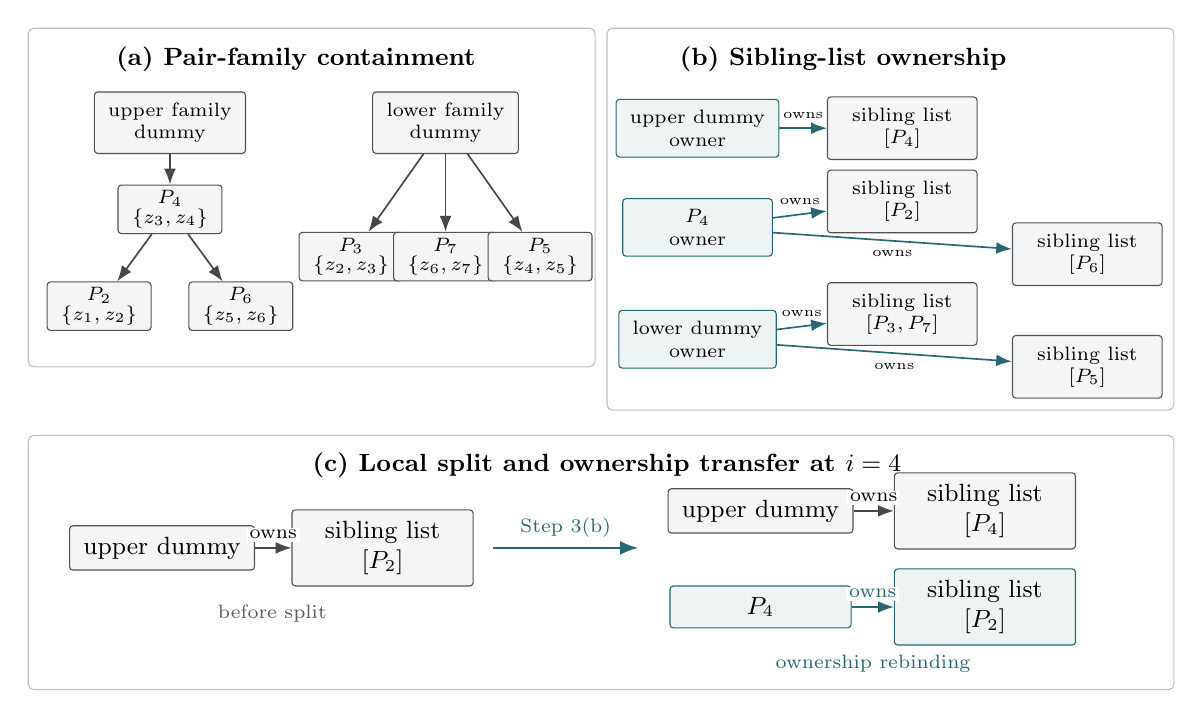
\begin{tikzpicture}[font=\small,node distance=7mm and 9mm]
  \node[font=\small\bfseries] at (3.05,4.95) {(a) Pair-family containment};
  \node[box,minimum width=1.55cm,font=\scriptsize] (ud) at (1.45,4.15)
    {upper family\\dummy};
  \node[box,minimum width=1.32cm,font=\scriptsize,inner xsep=2pt,inner ysep=2pt]
    (p4) at (1.45,3.05) {$P_4$\\[-1pt]$\{z_3,z_4\}$};
  \node[box,minimum width=1.32cm,font=\scriptsize,inner xsep=2pt,inner ysep=2pt]
    (p2) at (.55,1.82) {$P_2$\\[-1pt]$\{z_1,z_2\}$};
  \node[box,minimum width=1.32cm,font=\scriptsize,inner xsep=2pt,inner ysep=2pt]
    (p6) at (2.35,1.82) {$P_6$\\[-1pt]$\{z_5,z_6\}$};
  \draw[flow] (ud) -- (p4);
  \draw[flow] (p4) -- (p2);
  \draw[flow] (p4) -- (p6);

  \node[box,minimum width=1.55cm,font=\scriptsize] (ld) at (4.95,4.15)
    {lower family\\dummy};
  \node[box,minimum width=1.32cm,font=\scriptsize,inner xsep=2pt,inner ysep=2pt]
    (p3) at (3.75,2.45) {$P_3$\\[-1pt]$\{z_2,z_3\}$};
  \node[box,minimum width=1.32cm,font=\scriptsize,inner xsep=2pt,inner ysep=2pt]
    (p7) at (4.95,2.45) {$P_7$\\[-1pt]$\{z_6,z_7\}$};
  \node[box,minimum width=1.32cm,font=\scriptsize,inner xsep=2pt,inner ysep=2pt]
    (p5) at (6.15,2.45) {$P_5$\\[-1pt]$\{z_4,z_5\}$};
  \draw[flow] (ld) -- (p3);
  \draw[flow] (ld) -- (p7);
  \draw[flow] (ld) -- (p5);

  \node[font=\small\bfseries] at (10.0,4.95) {(b) Sibling-list ownership};
  \node[accent box,minimum width=1.9cm,font=\scriptsize] (uo) at (8.15,4.08) {upper dummy\\\scriptsize owner};
  \node[box,minimum width=1.9cm,font=\scriptsize] (ul) at (10.75,4.08) {sibling list\\$[P_4]$};
  \draw[accent flow] (uo) -- node[above,font=\tiny] {owns} (ul);

  \node[accent box,minimum width=1.9cm,font=\scriptsize] (p4o) at (8.15,2.82) {$P_4$\\\scriptsize owner};
  \node[box,minimum width=1.9cm,font=\scriptsize] (c1) at (10.75,3.15) {sibling list\\$[P_2]$};
  \node[box,minimum width=1.9cm,font=\scriptsize] (c2) at (13.10,2.48) {sibling list\\$[P_6]$};
  \draw[accent flow] (p4o) -- node[above,font=\tiny] {owns} (c1);
  \draw[accent flow] (p4o) -- node[below,font=\tiny] {owns} (c2);

  \node[accent box,minimum width=1.9cm,font=\scriptsize] (lo) at (8.15,1.40) {lower dummy\\\scriptsize owner};
  \node[box,minimum width=1.9cm,font=\scriptsize] (ll1) at (10.75,1.72) {sibling list\\$[P_3,P_7]$};
  \node[box,minimum width=1.9cm,font=\scriptsize] (ll2) at (13.10,1.05) {sibling list\\$[P_5]$};
  \draw[accent flow] (lo) -- node[above,font=\tiny] {owns} (ll1);
  \draw[accent flow] (lo) -- node[below,font=\tiny] {owns} (ll2);

  \node[font=\small\bfseries] at (7.0,-.20) {(c) Local split and ownership transfer at $i=4$};
  \node[box,minimum width=2.3cm] (beforeowner) at (1.35,-1.25) {upper dummy};
  \node[box,minimum width=2.3cm] (beforelist) at (4.15,-1.25) {sibling list\\$[P_2]$};
  \draw[flow] (beforeowner) --
    node[pos=.5,above=2pt,fill=white,inner sep=1pt,font=\scriptsize] {owns}
    (beforelist);
  \node[font=\scriptsize,text=black!65] at (2.75,-2.08) {before split};

  \draw[accent flow,line width=.8pt] (5.55,-1.25) -- node[above,font=\scriptsize,text=accent] {Step 3(b)} (7.40,-1.25);

  \node[box,minimum width=2.3cm] (afterowner) at (8.95,-.78) {upper dummy};
  \node[box,minimum width=2.3cm] (afterlist) at (11.80,-.78) {sibling list\\$[P_4]$};
  \draw[flow] (afterowner) --
    node[pos=.5,above=2pt,fill=white,inner sep=1pt,font=\scriptsize] {owns}
    (afterlist);
  \node[accent box,minimum width=2.3cm] (newowner) at (8.95,-2.00) {$P_4$};
  \node[accent box,minimum width=2.3cm] (newlist) at (11.80,-2.00) {sibling list\\$[P_2]$};
  \draw[accent flow] (newowner) --
    node[pos=.5,above=2pt,fill=white,inner sep=1pt,font=\scriptsize,text=accent] {owns}
    (newlist);
  \node[font=\scriptsize,text=accent] at (10.38,-2.72) {ownership rebinding};

  \begin{scope}[on background layer]
    \draw[black!25,rounded corners=2pt] (-.35,1.05) rectangle (6.85,5.35);
    \draw[black!25,rounded corners=2pt] (7.0,.50) rectangle (14.2,5.35);
    \draw[black!25,rounded corners=2pt] (-.35,-3.05) rectangle (14.2,.18);
  \end{scope}
\end{tikzpicture}
\end{document}
